\documentclass{article}
\usepackage[utf8]{inputenc}
\usepackage[spanish]{babel}
\usepackage{graphicx}
\graphicspath{ {images/} }
\begin{document}

\begin{titlepage}
    \begin{center}
        
        \huge
        \textbf{¿Por que hay tantos tipos de memoria? si su utilidad es solo una}
        \large 
        
        \vspace{1cm}
        ¿Para que sirven tantos tipos de memoria?
        \vspace{4cm}
        
        Daniel Cano Restrepo
        
        \vspace{9cm}
        
        \small
        Despartamento de Ingeniería Electrónica y Telecomunicaciones\\
        Universidad de Antioquia\\
        Medellín\\
        Septiembre de 2020
        
    \end{center}
\end{titlepage}

\tableofcontents



\newpage
\section{Introducción}

\vspace{1cm}
En una computadora se encuentran varios tipos de memoria, la ram, la caché, la virtual, etc; entonces al escuchar tantas variedades y nombres uno se pregunta ¿para qué tantas? si la memoria es tan solo algo para guardar cosas. Y claro! si las cosas se plantean así, no se entiende el porque fue diseñado un computador de esta manera, por esto primero debemos conocer cada una de las memorias y sus características, y así entender la importancia que tiene cada una de ellas dentro en un computador.

\vspace{3cm}

\section{¿Cuáles son los tipos de memoria y que función tienen?}
\vspace{1cm}
\begin{center}
    \textbf{SSD o HDD}
\end{center}

Este par de memorias tienen un funcionamiento diferente pero cumplen la misma función, y es guardar información de manera permanente.
\vspace{0.4cm}


El disco duro (HDD) hace esto mediante unos discos que guardan la información en forma de campo magnético, el HDD suele ser la memoria más lenta dentro de una computadora, pero la de mayor tamaño.\cite{ssd}
\vspace{0.4cm}

\begin{figure}
    \centering
    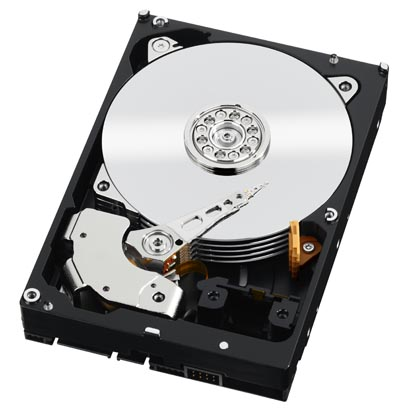
\includegraphics[width=4cm]{HDD.png}
    \caption{HDD}
    \label{fig:my_label}
\end{figure}[h]


La SSD es una memoria más veloz que el HDD, sin partes mecánicas, más resistentes a golpes que los HDD…, hasta le gana en precio!; pero ya fuera de bromas esta tecnología es relativamente nueva y muy buena, su única pega es que no posee una durabilidad ni un tamaño tan alto como el de un disco duro. Su funcionamiento está basado en celdas donde se guarda la información, que a su vez están dentro de unos bloques. Esta estructura le permite ser más veloz.\cite{disco}

\begin{figure}
    \centering
    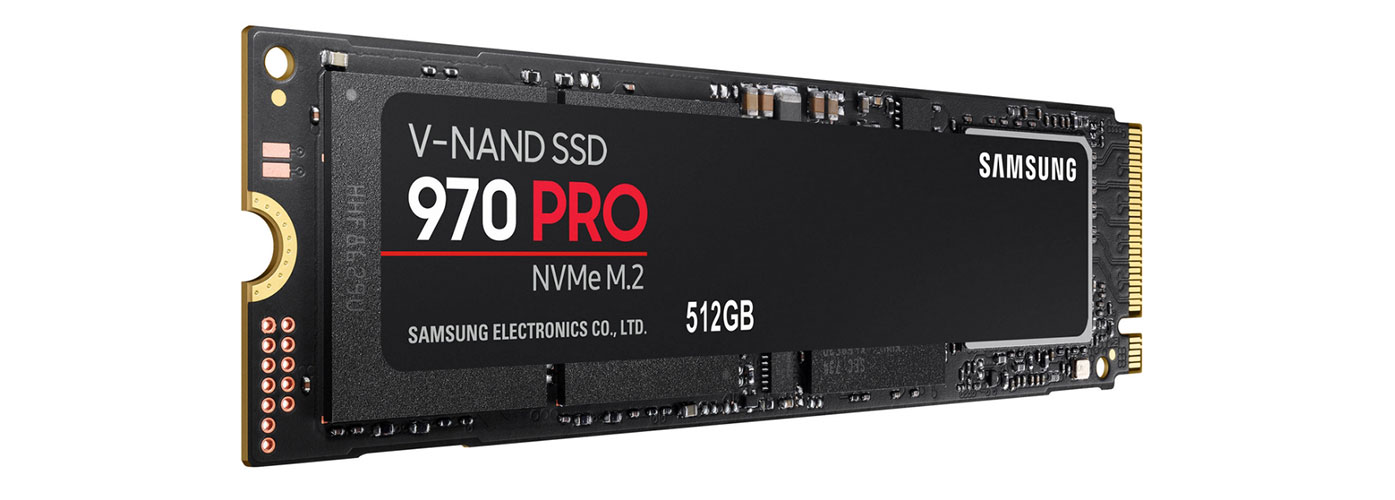
\includegraphics[width=4cm]{SSD.jpg}
    \caption{SDD}
    \label{fig:my_label}
\end{figure}

\vspace{3cm}
\begin{center}
    \textbf{RAM (DRAM)}
\end{center}
La ''RAM'' es una memoria muy famosa, todos nos fijamos en ella al comprar una computadora, esta memoria es mucho mas rapida que las anteriores, y cuando digo mucho es \textbf{MUCHO}, esto se da por que la RAM tiene la capacidad de acceder a la información instantáneamente sin importar su ubicación, pero por mas rapida que sea tiene un pequeño detalle, y es que al apagar el computador la información dentro de la RAM desaparece, esto se da ya que está hecha de capacitores(son como contenedores de electrones) los cuales tienen fugas de electrones, si el capacitor se llega a vaciar un 1 se convertirá en 0,  por ende la información se vería corrompida y el windows no te correria(bromas aparte, esto hace que estos capacitores constantemente sean rellenados). esta memoria es mucho más cara que las anteriores y se suele encontrar en tamaños mucho más reducidos (nunca he visto una que pase de las 100gb).\cite{pdfu}
\begin{figure}
    \centering
    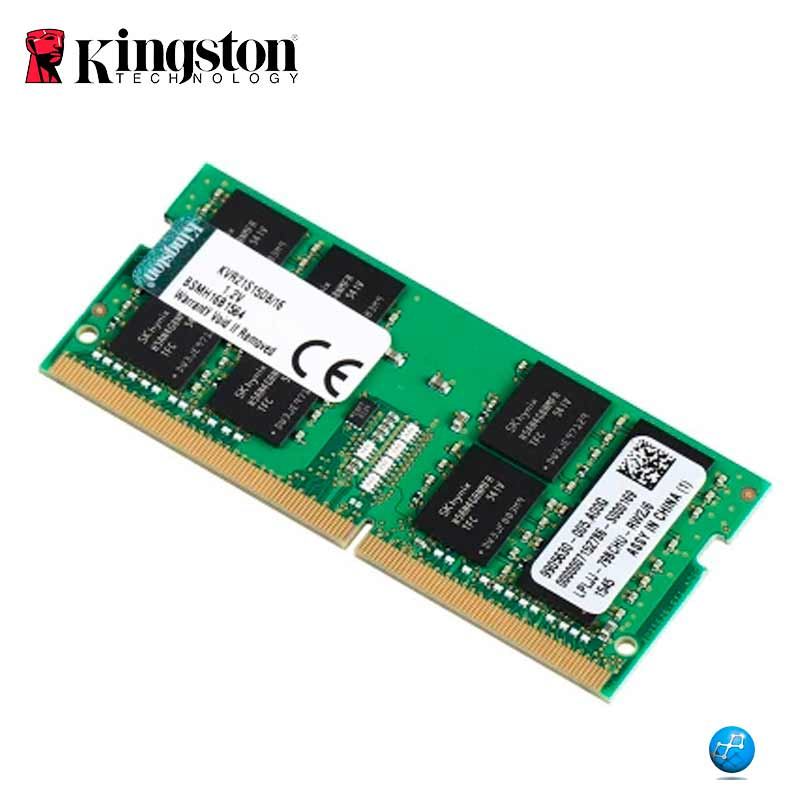
\includegraphics[width=4cm]{RAM.jpg}
    \caption{RAM}
    \label{fig:my_label}
\end{figure}

\vspace{5cm}

\begin{center}
    \textbf{CACHE (SRAM)}
\end{center}

\vspace{1cm}
Esta memoria es muy parecida a la RAM solo que en esta por medio de unos transistores logra que dicha fuga de electrones no se de con regularidad, y con esto logra una velocidad mucho mayor que la de la RAM. Este tipo de memoria se encuentra dentro del procesador y se divide en 3 niveles (L1, L2, L3) a más pequeño el número más veloz ma memoria, L1 y L2 se encuentran dentro de cada núcleo del CPU, L3 es una memoria para todos los núcleos de la cpu, esta memoria es la mas rapida dentro de un computador. \cite{pdfu} 
\vspace{3cm}

\section{Gestión de memorias dentro de un computador}
\vspace{1cm}

Ya que entendimos las características de cada una, estamos listos para entender cómo funcionan en conjunto, para lograr entender porque las cosas se organizan así, hay que entender los problemas que nos llevaron a requerir dicha organización.
\vspace{0.4cm}

Pensemos que queremos abrir un archivo, al nosotros darle la orden al computador de que abra dicho archivo, el instantáneamente manda una señal al HDD o SSD pidiendo el archivo y la aplicación con las instrucciones para manejar dicho archivo, para luego guardar la aplicación y el archivo en la RAM,¿por que no pasa a la cpu directamente? por que el disco duro va tan lento que se desaprovecha el potencial de la cpu, en la RAM se coloca el archivo y las partes de la app fundamentales para su funcionamiento, como la ram tampoco es suficiente para poder saciar al procesador, se colocan los archivos mas usados dentro de la cache, entonces ¿por qué no nos armamos una computadora con solo cache y SSD? Primero porque la caché es mucho más cara que la RAM, segundo la caché ocupa mucho más espacio que la RAM, entonces la función queda muy clara.\cite{pdfu}
\vspace{0.4cm}

\textbf{SSD o HDD:} donde se guardan los archivos permanentes de la 
computadora.
\vspace{0.4cm}

\textbf{RAM:} donde se guardan los archivos que se van a usar próximamente.
\vspace{0.4cm}

\textbf{Memoria virtual:} esta memoria aparece en caso tal que la memoria RAM haya sido totalmente ocupada, si esto pasa se abrirá un espacio en el disco duro para que sea como el suplente de la memoria RAM(con la consecuencia de que el computador irá más lento).
\vspace{0.4cm}

\textbf{Caché:} es la memoria donde se guardan los archivos mas usados por el procesador. 
\vspace{3cm}
\newpage
\section{Conclución}
\vspace{1cm}
El que haya tantos tipos de memorias en el mundo de los computadores de hoy en día, es una consecuencia directa de los límites físicos, monetarios y creativos que poseemos, quien sabrá si en futuro los tendremos, pero por ahora es bueno conocerlos para solucionarlos.
\vspace{3cm}



\bibliographystyle{IEEEtran}
\bibliography{biblio}





\end{document}
